%%%%%%%%%%%%%%%%%%%%%%%%%%%%%%%%%%%%%%%%%%%%%%%%%%%%%
%			CELÝ ZPĚVNÍK v. 18.09  					%
%%%%%%%%%%%%%%%%%%%%%%%%%%%%%%%%%%%%%%%%%%%%%%%%%%%%%
% Toto je hlavní soubor zpěvníku, z kterého lze 
% kompilovat celý zpěvník se všemi písničkami.
%%%%%%%%%%%%%%%%%%%%%%%%%%%%%%%%%%%%%%%%%%%%%%%%%%%%%
%			Jak kompilovat celý zpěvník?			%
%%%%%%%%%%%%%%%%%%%%%%%%%%%%%%%%%%%%%%%%%%%%%%%%%%%%%
% Přidání nové písničky probíhá tak, že:
% 1. Napíšete .tex soubor s textem písničky a akordy 
% a soubor vložíte do ../songy
%	a) Soubor se píše podle pravidel napsaných 
%	   v souboru ../Generator/generator.tex
%	b) V souboru ../Generator/generator.tex
%	   se soubor také kompiluje samostatně 
%      pro kontrolu.
% 2. Písnička se přidá na místě označeném kódem 
%    PRIDAVANI (ctrl+f a dá se to najít). Přidáte 
%    ji vložením následujícího řádku podle abecedy: 
%    \addcontentsline{toc}{section}{[ZDE NAPIŠ NÁZEV PÍSNIČKY]}\input{../songy/[ZDROJOVÝ SOUBOR PÍSNIČKY].tex}\newpage
% 3. Výsledek s zobrazí po kompilaci DVAKRÁT 
%    za sebou (kvůli toc).
% (4.) Předmluva se upravuje na místě PŘEDMLUVA.
% (5.) Cover obrázek: PŘEBAL1
% (6.) Watermark: VODOZNAK
% (7.) Seznam všech akordů: PŘEHLED
%%%%%%%%%%%%%%%%%%%%%%%%%%%%%%%%%%%%%%%%%%%%%%%%%%%%%
%			Jak kompilovat jednotlivé písně?        %
%%%%%%%%%%%%%%%%%%%%%%%%%%%%%%%%%%%%%%%%%%%%%%%%%%%%%
%	1. Více návodu je k tomuto napsáno v souboru 
%      ../Generator/generator. 
%%%%%%%%%%%%%%%%%%%%%%%%%%%%%%%%%%%%%%%%%%%%%%%%%%%%%
%			Jak psát soubory songů?                 %
%%%%%%%%%%%%%%%%%%%%%%%%%%%%%%%%%%%%%%%%%%%%%%%%%%%%%
%	1. Více návodu je k tomuto napsáno v souboru 
%      ../songy/00Songtemplate. 
%%%%%%%%%%%%%%%%%%%%%%%%%%%%%%%%%%%%%%%%%%%%%%%%%%%%%

\documentclass[openany,12pt]{memoir}
\usepackage[utf8]{inputenc}
\usepackage[czech]{babel}
\usepackage[T1]{fontenc}
\usepackage[top=1.5cm, bottom=2cm, left=2cm, right=2cm]{geometry}  % --> NASTAVENÍ OKRAJŮ
\usepackage{fancyhdr}
\usepackage{graphicx}
\usepackage{xwatermark}
\usepackage{xcolor}
\usepackage{changepage}
\usepackage{pdfpages}
\usepackage{lettrine}
\usepackage{indentfirst}  %Důležité pro formátování
\usepackage[pages=some]{background}

%%%%%%%%%%%%%%%%%%%%%%%%%%%%%%%%%%%%%%
%  FONT                              %
%%%%%%%%%%%%%%%%%%%%%%%%%%%%%%%%%%%%%%
\usepackage{amssymb}
\usepackage{tgschola}

%%%%%%%%%%%%%%%%%%%%%%%%%%%%%%%%%%%%%%
%  Obrázky v textu                   %
%%%%%%%%%%%%%%%%%%%%%%%%%%%%%%%%%%%%%%
\usepackage{tikz}
%\tikz[remember picture,overlay] \node[opacity=0.3,inner sep=0pt] at (current page.center){\includegraphics[width=\paperwidth,height=\paperheight]{example-image}};
%Tímto příkazem se na následující stránku vloží pozadí. Pokud pozadí uděláme
%tak, aby bylo velikosti a4, bylo prázdné až na malůvku, můžeme takto vkládat
%obrázky.
%Pozn.: kompilovat se musí dvakrát


%%%%%% Package na zpěvník
\usepackage[full]{leadsheets}%http://mirrors.nic.cz/tex-archive/macros/latex/contrib/leadsheets/leadsheets_en.pdf   --> dokumentace	
\definesongtitletemplate{empty}{} 
\setchords{
format = \bfseries \sffamily,   %tučné akordy
minor = {mi},% 
input-notation = {german},%
output-notation = {german}%
}
\definesongtitletemplate{empty}{} 

\newlength{\drop}
% VODOZNAK
\newwatermark[pages=3-,color=red!50,angle=0,scale=2, xpos=0,ypos=0]{
\includegraphics[width=5cm]{obr/pozadi2.jpg}} %--> dvojka na pozadí


%%%%%%%%%%%%%%%%%%%%%%%%%%%%%%%%%%%%%%%%%%%%%%%%%%
%		 Vlastní příkazy
\newcounter{Slokočet}   %Automatické číslování slok
\newcommand{\mezera}{
\phantom{.}

}   %Horizontální odsazení slok (poněkud blbě zadefinovaný, ale jinak se formát rozbije jako wtf prostě)
\newcommand{\stred}{5.2cm}   %%% Na zarovnání slok doprostřed, pozn. automatičtější zarovnávání na střed nejde
\newcommand{\carka}{,\:}
\newcommand{\m}[1]{\color{white}{#1}}  %Pro akordy
\newcommand{\ap}{'}	%Pro apostrof
\newcommand{\elipsa}{\kern\fontdimen3\font} %Příkaz pro lepší zacházení s výpustkami (=...); je to vpodstatě jen mezera mezi tečkama výpustky
\newcommand{\pindent}{17.62482 pt} %Správná velikost \parindentu u layoutu se dvěma minipageama
\newcommand{\predtitle}{\huge}
\newcommand{\mezisloupci}{\phantom{TT}} %Místo mezi dvěma sloupci na jedné stránce
\newcommand{\z}{\hspace*{\fill}\null}

%%% Možné velikosti písem 
\newcommand{\normalni}{\normalsize}
\newcommand{\velky}{\fontsize{14.4}{15}\selectfont}
\newcommand{\vetsi}{\fontsize{15}{16}\selectfont}
\newcommand{\nejvetsi}{\fontsize{16}{17}\selectfont}
\newcommand{\nejnejvetsi}{\fontsize{17}{19}\selectfont}

%%% Stará definice sloky spoléhající na indenty
%\newlength{\pismeno}
%\settowidth{\pismeno}{x} %Tohle není moc ideální velikost, ale funguje
%\newif\ifslokavelka
%\slokavelkafalse
%\newcommand{\sloka}{
%\ifnum \value{Slokočet}>8  %Pokud je sloka dvouciferná
%\mezera \noindent \addtocounter{Slokočet}{1} \hspace*{-\pismeno}\arabic{Slokočet}.
%\else %Pokud jen jednociferná
%\mezera \noindent \addtocounter{Slokočet}{1} \arabic{Slokočet}. 
%\fi
%} 	%sloka, která se automaticky čísluje

\newcommand{\distanc}{\:}  %Vzdálenost čísla sloky před slokou
\newlength{\delkaargumentu}
%%% Sloka s automatickým číslováním
\newcommand{\sloka}{%
\addtocounter{Slokočet}{1}% Zvýší se o 1 počet slok
\mezera%  Sloka se odsadí vertikálně
\settowidth{\delkaargumentu}{\arabic{Slokočet}.\distanc}% Zde se určí délka odsazení 
\hspace*{-\delkaargumentu}%
\arabic{Slokočet}.\distanc%
\ignorespaces% Aby nevznikaly zbytečné mezery
}


%%% Sloka s vlastním argumentem
\newcommand{\ssloka}[1]{%     
\settowidth{\delkaargumentu}{#1\distanc}
\mezera%
\hspace*{-\delkaargumentu}%
#1\distanc%
\ignorespaces%
}  

%%% Refrén
\newcommand{\refren}[1][0]{%  Nepovinný argument sděluje, kolikátý refrén toto je, bez argumentu se vytiskne pouze refrén
\ifnum #1>0 %Pokud nepovinný argument existuje
\mezera%
\settowidth{\delkaargumentu}{\textbf{R$_{\text{#1}}$:}\distanc}%
\hspace*{-\delkaargumentu}%
\textbf{R$_{\text{#1}}$:}\distanc%
\ignorespaces%
\else %Pokud nepovinný argument neexistuje
\mezera%
\settowidth{\delkaargumentu}{\textbf{R:}\distanc}%
\hspace*{-\delkaargumentu}%
\textbf{R:}\distanc%
\ignorespaces%
\fi
}

\newcommand{\predehra}{\ssloka{\textbf{Předehra:}}}

%%% Capo
\newcommand{\kapodastr}[1]{
\textit{Capo \text{#1}}
}

\addto\captionsczech{\renewcommand{\contentsname}{Seznam písní}}

%%%%%%%%%%%%%%%%%%%%%%%%%%%%%%%%%%%%
%    FORMÁTOVÁNÍ                   %
%%%%%%%%%%%%%%%%%%%%%%%%%%%%%%%%%%%%

%%% Vlevo zarovnaný text s blokem zarovnaným na střed
\usepackage{varwidth}% http://ctan.org/pkg/varwidth
\newenvironment{centerjustified}{%
  \begin{center} % so the minipage is centered
  \begin{varwidth}[t]{\textwidth}	
  \raggedright % so the minipage's text is left justified
  \setlength{\parindent}{\pindent}
}{%
  \end{varwidth}
  \end{center}
}

%%% Pozadí
\newcommand{\pozadi}[1]{
\backgroundsetup{
scale=1,
angle=0,
contents={%
  \includegraphics[width=\paperwidth,height=\paperheight]{#1}
  }%
}
\BgThispage
}




\usepackage{hyperref} %Musí být načteno jako poslední package
\begin{document}
\sffamily %Sans-serif font vypadá lépe
\velky   %Minimální čitelná velikost


\renewcommand{\abstractname}{\vspace{-\baselineskip}} %Aby nad úvodním textem nebyl nápis ,,Abstract''


%Kompilovat dvakrát, aby se updatnula TOC

\setcounter{page}{0}
\pagestyle{empty}
%%%%%%%%%%%% PŘEBAL1 %%%%%%%%%%%%%%%%%%
\includepdf[width=\paperwidth]{obr/Prebal_2020.png}
\newpage
\phantom{prázdná strana}
\newpage

%%%%%%%%%%%% Úvod %%%%%%%%%%%%%%%%%%
\vspace*{4\baselineskip}
\begin{abstract}
\large 

\sffamily
% PŘEDMLUVA
\lettrine{P}{}rávě se k Vám dostal další z řady oddílových zpěvníků
\textbf{Pražské Dvojky}. Tento zpěvník si klade za cíl být striktně lepší
náhradou nynějších zpěvníků jakéhokoliv druhu poskytující všemožné designové
a~funkční vylepšení (umožněné programem \LaTeX ).\\
Najdete tu značné množství písniček, které tvůrci považují za hodící se k~ohni
s~kytarou i~s~akordy na kytaru. Kromě táborákových evergreenů a aktuálních hitů
jsme do zpěvníku zapracovali i~historické verze Dvojkařských písniček, které se
přes svojí přitažlivost, exotiku a romantiku jen zřídka vyskytují v~ostatních
zdrojích.\\
V případě, že ve zpěvníku naleznete nesrovnalosti nebo byste do něj chtěli
přidat další píseň, rádi Vaše připomínky zapracujeme do budoucích verzí
zpěvníku.
Kód zpěvníku je k~dispozici i~na \href{https://github.com/JindrazPrahy/DvojkarskyZpevnik}{GitHubu}. \\ \\
Za úvodní kresbu na přebalu děkujeme \textbf{Pavoukovi}. Obrázky akordů
používáme ze stránky \href{https://jguitar.com/}{www.jguitar.com}.\\\\\\\\\\
Hodně zábavy při zpěvu přejí tvůrci zpěvníku\\\\
\textbf{Jindra} \& \textbf{Albert}.\\\\\\\\\\\\\\\\\\\\
{\tiny \rmfamily Zpěvník 20.06, Ctižádostivý cejn LTS}
\end{abstract}
\newpage


%%%%%%%%%%%%% Písně %%%%%%%%%%%%%%%%
%% Okraje:
% P+L = 4cm
% T = 1.5cm
% B = 0 cm

\newgeometry{top=1.5cm, bottom=2cm, left=2cm, right=2cm}
\setlrmarginsandblock{1cm}{3cm}{*} %Kvůli dírám pro kroužky
\setulmarginsandblock{1.5cm}{1cm}{*}
\checkandfixthelayout

%%%%%%%%%%%%% Obsah %%%%%%%%%%%%%%%%
\addtocontents{toc}{\protect\thispagestyle{empty}}
\tableofcontents* \thispagestyle{empty}\newpage
\newgeometry{top=1.5cm, bottom = 0cm, left = 2cm, right = 2cm}
\setlrmarginsandblock{1cm}{3cm}{*} %Kvůli dírám pro kroužky
\setulmarginsandblock{1.5cm}{0cm}{*}
\checkandfixthelayout 



% PRIDAVANI

\newcommand{\importsong}[2]{\phantomsection\addcontentsline{toc}{section}{#1}\input{../songy/#2}\newpage}

\pagestyle{simple}
\importsong{Skautská hymna a Večerka}{0SkautskaHymna.tex}
\importsong{1. signální}{1signalni.tex}
\importsong{All Stars}{AllStars.tex}
\importsong{Always Look On The Bright Side Of Life}{AlwaysLookOnTheBrightSideOfLife.tex}
\importsong{Amerika}{Amerika.tex}
\importsong{Anděl}{Andel.tex}
\importsong{Andělská}{Andelska.tex}
\importsong{Ani k stáru}{AniKStaru.tex}
\importsong{Antidepresivní rybička}{AntidepresivniRybicka.tex}
\importsong{Bastila}{Bastila.tex}
\importsong{Batalion}{Batalion.tex}
\importsong{Bonanza}{Bonanza.tex}
\importsong{Boží vlak}{BoziVlak.tex}
\importsong{Bujonet}{Bujonet.tex}
\importsong{Carpe Diem}{CarpeDiem.tex}
\importsong{Cestou do Jenkovic}{CestouDoJenkovic.tex}
\importsong{Cestou od hřbitova}{CestouOdHrbitova.tex}
%% ABECEDNÍ POŘADÍ PROHOZENO, ABY DVOJSTRANNÁ PÍSNIČKA BYLA HRATELNÁ BEZ OTOČENÍ STRÁNK
\importsong{Counting Stars}{CountingStars.tex} % 2-stranna verze
\importsong{Cigarette Daydreams}{CigaretteDaydreams.tex}
\importsong{Černej pasažér}{CernejPasazer.tex}
\importsong{Černobílý svět}{CernobilySvet.tex}
\importsong{Danse macabre}{DanseMacabre.tex}
\importsong{Darmoděj}{Darmodej.tex}
\importsong{Dej mi víc své lásky}{DejMiVicSveLasky.tex}
\importsong{De N\^{i}mes}{DeNimes.tex}
\importsong{Dezolát}{Dezolat.tex}
\importsong{Dirty Paws}{DirtyPaws.tex}
\importsong{Do Ameriky}{DoAmeriky.tex}
\importsong{Do dne a do roka}{DoDneADoRoka.tex}
\importsong{Dokud se zpívá}{DokudSeZpiva.tex}
\importsong{Dopis}{Dopis.tex}
\importsong{Ekosong}{Ekosong.tex}
\importsong{Franky Dlouhán}{FrankyDlouhan.tex}
\importsong{God\ap s Gonna Cut You Down}{GodsGonnaCutYouDown.tex}
\importsong{Hallelujah}{Hallelujah.tex}  % Pouze jednostranná verze
\importsong{Hercegovina}{Hercegovina.tex}
\importsong{Hero of War}{HeroofWar.tex}
\importsong{Hey Ho}{HeyHo.tex}
\importsong{Hlídač krav}{HlidacKrav.tex}
\importsong{Hodinový hotel}{HodinovyHotel.tex}
\importsong{Homosexuál}{Homosexual.tex}
\importsong{Hotel Hillary}{HotelHillary.tex}
\importsong{Houpej se člunku malý}{HoupejSeClunku.tex}
\importsong{House Of The Rising Sun}{HouseOfTheRisingSun.tex}
\importsong{Housličky}{Houslicky.tex}
\importsong{Hruška}{Hruska.tex}
\importsong{Hudsonský šífy}{HudsonskeSify.tex}
\importsong{Hurt}{Hurt.tex}
\importsong{Hvězdář}{Hvezdar.tex}
\importsong{Chci ti říct}{ChciTiRict.tex}
\importsong{I cesta může být cíl}{ICestaMuzeBytCil.tex}
\importsong{I\ap m gonna be 500 miles}{ImGonnaBe500Miles.tex}
\importsong{Indian}{Indian.tex}
\importsong{Jdem zpátky do lesů}{JdemZpatkyDoLesu.tex}
\importsong{Je jaká je}{JeJakaJe.tex}
\importsong{Ještě jedno kafe}{JesteJednoKafe.tex}
\importsong{John Brown}{JohnBrown.tex}
\importsong{Kaliforňané}{Kalifornane.tex}
\importsong{Kamarádi}{Kamaradi.tex}
\importsong{Karavana mraků}{KaravanaMraku.tex}
\importsong{Kluziště}{Kluziste.tex}
\importsong{Knocking On Heaven\ap s Door}{Knockin.tex}
\importsong{Kometa}{Kometa.tex}
\importsong{Kovárna}{Kovarna.tex}
\importsong{Král a klaun}{KralAKlaun.tex}
\importsong{Kutil}{Kutil.tex}
\importsong{Lano, co k nebi nás poutá}{LanoCoKNebiNasPouta.tex}
\importsong{Laudato sii}{LaudatoSii.tex}
\importsong{Leaving On A Jet Plane}{LeavingOnAJetPlane.tex}
\importsong{Lemon Tree}{LemonTree.tex}
\importsong{Let Her Go}{LetHerGo.tex} %2-stranna
\importsong{Let It Be}{LetItBe.tex}
\importsong{Letím hledat světy}{LetimHledatSvety.tex}
\importsong{Lilie}{Lilie.tex}
\importsong{Lišaji}{Lisaji.tex}
\importsong{Little Talks}{LittleTalks.tex}
\importsong{Loďka Malá}{LodkaMala.tex}
\importsong{Lokomotiva}{Lokomotiva.tex}
\importsong{Made in Valmez}{MadeInValmez.tex}
\importsong{Mám doma kočku}{MamDomaKocku.tex}
\importsong{Mezi Horami}{MeziHorami.tex}
\importsong{Měsíc}{Mesic.tex}
\importsong{Milionář}{Milionar.tex}
\importsong{Milionář II}{Milionar2.tex}
\importsong{Mladičká básnířka}{MladickaBasnirka.tex}
\importsong{Modlitba pro partu}{ModlitbaProPartu.tex}
\importsong{Muzeum}{Muzeum.tex}
\importsong{Nad stádem koní}{NadStademKoni.tex}
\importsong{Nagasaki Hirošima}{NagasakiHirosima.tex}
\importsong{Nebe peklo ráj}{NebePekloRaj.tex}
\importsong{Nebeští jezdci}{NebestiJezdci.tex} 
\importsong{Nejlíp jim bylo}{NejlipJimBylo.tex}
\importsong{Nezacházej slunce}{NezachazejSlunce.tex}
\importsong{One}{One.tex} % 2-stranna
\importsong{Orlice}{Orlice.tex}
\importsong{Osmá barva duhy}{OsmaBarvaDuhy.tex}
\importsong{Ostravo}{OstravoOstravo.tex}
% \phantomsection\addcontentsline{toc}{section}{Otevřená zlomenina srdečního svalu}\begin{song}{title=\predtitle\centering Otevřená zlomenina srdečního svalu \\\large Wanastowi Vjecy \vspace*{-0.3cm}}  %% sem se napíše jméno songu a autor
\begin{centerjustified}

\sloka 
	Jsem jako ^{G\,\,}vítr kterej zfoukne pírko ze tvejch dlaní,

	^{D{\color{white}\_\_}}špínu jedný noci, jako hygiena ranní,

	^{Ami}velká voda slzí, který spláchnou noční hříchy, 

	^{C{\color{white}\_\_\_\_}}tamburíny zvoní k ^{Es7{\color{white}\_\_}}operaci míchy.
	
	^{\phantom{.}}Narovnám ti páteř, poškrábu ti záda, 
	
	pofoukám ti srdce, zrada kamaráda

	lásky účel světí prostředky a smetí, 
	
	špínu jedný noci, který neuletíš.

	Otevřená zlomenina srdečního svalu, 
	
	trápení a kocovina, vůně tvýho žalu.
	
	Vypustíš svou hříšnou duši do slanýho moře, 
	
	neumírej děvče moje, chci ti říct že:


\refren
	Ohořelou ^{G{\color{white}\_\_}}károu chtěl bych dojet ^{D}ke hvězdám,

	který ^{Ami}svítily z tvejch očí ^{C{\color{white}\_}}dřív než červotoči 

	se do tvýho srdce ^{F}daj, hm ^{D}hm.
	
	^{\phantom{.}}V ohořelym autě už dva měsíce nedejchám,
	
	sám se svojí vinou, už nikdy nechci jinou, 
	
	už asi nedoufám.

\sloka
	Pláčem solíš otevřený rány co se hojí, 
	
	tvoji krev i tělo příjímám pod obojí.

	Stejný lidi se soumrakem mají stejný stíny, 
	
	zmizelas jak před přízrakem, padám do hlubiny.
	
	Tvůj pramínek vlasů zaliju včelím voskem, 
	
	koukám na tu krásu a nechápu to mozkem.
	
	To co jsi mi dala já nikomu už nedám, 
	
	tak mi řekni má opičko proč tě marně hledám.

	Otevřená zlomenina srdečního svalu, 
	
	trápení a kocovina, vůně tvýho žalu.
	
	Vypustíš svou hříšnou duši do slanýno moře, 

	neumírej děvče moje, chci ti říct, že:

\refren



\end{centerjustified}
\setcounter{Slokočet}{0}
\end{song}
\newpage % Nehrajem
\importsong{Pangajó}{Pangajo.tex}
\importsong{Partyzán}{Partyzan.tex}
\importsong{Passenger}{Passenger.tex}
\importsong{Pažitka}{Pazitka.tex}
\importsong{Perfect Day}{PerfectDay.tex}
\importsong{Personal Jesus}{PersonalJesus.tex}
\importsong{Petěrburg}{Peterburg.tex}
\importsong{Pijánovka}{Pijanovka.tex}
\importsong{Písnička pro Tebe}{PisnickaProTebe.tex}
\importsong{Pocity}{Pocity.tex}
\importsong{Podzimní}{Podzimni.tex}
\importsong{Pohádka}{Pohadka.tex}
\importsong{Pohár a Kalich}{PoharAKalich.tex}
\importsong{Pověste ho vejš}{PovesteHoVejs.tex}
\importsong{Proklatej vůz}{ProklatejVuzVerII.tex}
\importsong{Pro malou Lenku}{ProMalouLenku.tex}
\importsong{Převrat v Banánové republice}{PrevratVBananoveRep.tex}
\importsong{Pyšný Janek} {PysnyJanek.tex}
\importsong{Ráda se miluje}{RadaSeMiluje.tex}
\importsong{Radioactive}{Radioactive.tex}
%\addcontentsline{toc}{section}{Rád vařim}%\documentclass[../main.tex]{subfiles}

\newcommand\tab[1][1cm]{\hspace*{#1}}
\begin{song}{title=\centering Rád vařim \\\normalsize MIDI LIDI \vspace*{-0.3cm}}  %% sem se napíše jméno songu a autor
\moveright 1cm \vbox{      %Varianta č. 1  ---> Jeden sloupec zarovnaný na střed	
\begin{minipage}[t]{0.48\textwidth}\setlength{\parindent}{0.45cm}  %Varianta č. 2 --> Dva sloupce

\sloka
^{Gmi}Rád ^{Cmi\,\,\,\,}vařim a ^{Gmi\,\,}vim, že to ^{Cmi\,\,\,\,}umim

a ^{Gmi\,\,\,\,\,\,\,\,}holkám ^{Cmi}se to ^{Dmi}líbí.

\phantom{.}

Rád vařím a vím, že to umím

a holkám se to líbí.

\phantom{.}

Rád vařím a vím, že to umím

a holkám se to líbí.

\phantom{.}

Rád vařím a vím, že to umím

a holkám se to líbí.

\phantom{.}

[Mezihra]

\sloka
Rád vařím a vím, že to umím

a holkám se to líbí.

\phantom{.}

Rád vařím a vím, že to umím

a holkám se to líbí.

\phantom{.}

Rád vařím a holkám vařím 

a holkám se to líbí.

\phantom{.}

Já rád vařím a holkám vařím 

a holkám se to líbí.


\sloka
Rád vařím a holkám vařím
 
a holkám se to líbí.

\phantom{.}

Rád vařím a holkám vařím 

a holkám se to líbí.

\phantom{.}

Já vařím a holkám vařím
 
a holkám se to líbí.

\phantom{.}

Rád vařím a holkám vařím 

a holkám se to líbí.

\phantom{.}

[Mezihra]

\end{minipage}\begin{minipage}[t]{0.48\textwidth}\setlength{\parindent}{0.45cm}\vspace*{0.55cm}  % V případě varianty č.2 jde odsud text do pravé části

\sloka
Rád vařím a vím, že to umím

a holkám se to líbí.

\phantom{.}

Rád vařím a holkám vařím 

a moc se mi to líbí.

\phantom{.}

Rád mlčím a doma trčím 

ale v práci mi to myslí.

\phantom{.}

Rád mlčím a doma trčím 

ale v práci mi to myslí.

\phantom{.}

Rány hojím, a proto za to stojím

a Vám všem se to líbí.

\phantom{.}

Rány hojím, a proto za to stojím 

a Vám všem se to líbí.

\end{minipage}
}
\setcounter{Slokočet}{0}
\end{song}
\newpage % Tezko se hraje
\importsong{Russian mystic pop IV.}{RussianMysticPopIV.tex}
\importsong{Řekni, kde ty kytky jsou}{RekniKdeTyKytkyJsou.tex} %carka v nazvu
\importsong{Riptide}{Riptide.tex} %carka v nazvu
\importsong{Rodné údolí}{RodneUdoli.tex} %carka v nazvu
\importsong{Sametová}{Sametova.tex}
\importsong{Sarajevo}{Sarajevo.tex}
\importsong{Sáro!}{Saro.tex}
\importsong{Severní vítr}{SeverniVitr.tex}
\importsong{Shotgun}{Shotgun.tex}
\importsong{Slaboch Ben}{SlabochBen.tex}
\importsong{Sladké mámení}{SladkeMameni.tex}
\importsong{Slavíci z Madridu}{SlaviciZMadridu.tex}
\importsong{Slova}{Slova.tex}
\importsong{Slunečný hrob}{SlunecnyHrob.tex}
\importsong{Soudný Den}{SoudnyDen.tex}
\importsong{Sound Of Silence}{SoundOfSilence.tex}
\importsong{Space Oddity}{SpaceOddity.tex} % 2-stranna
\importsong{Stánky}{Stanky.tex}
\importsong{Staré dobré časy}{StareDobreCasy.tex}
\importsong{Stín}{Stin.tex}
\importsong{Strom kýve pahýly}{StromKyvePahyly.tex}
\importsong{Studený nohy}{StudenyNohy.tex}
\importsong{Svatební}{SvatebniNohav.tex}
\importsong{Svatební píseň}{SvatebniJarda.tex}
\importsong{Své Rocky Mountains}{SveRockyMountains.tex}
\importsong{To ta He\v lpa}{ToTaHelpa.tex}
\importsong{Traktor}{Traktor.tex}
\importsong{Trezor}{Trezor.tex}
\importsong{Tu kytaru jsem koupil kvůli tobě}{TuKytaruJsemKoupil.tex}
\importsong{Už slyším Boží mlýny}{UzSlysimBoziMlyny.tex}
\importsong{Už to nenapravím}{UzToNenapravim.tex}
\importsong{Včelka Mája}{VcelkaMaja.tex}
\importsong{Veličenstvo Kat}{VelicenstvoKat.tex}
\importsong{Velmi nesmělá}{VelmiNesmela.tex}
\importsong{Ve skříni}{VeSkrini.tex}
\importsong{Věděl pan Cicero}{VedelPanCicero.tex}
\importsong{V jejích šlépějích}{VJejichSlepejich.tex}
\importsong{Vlachovka}{Vlachovka.tex}
\importsong{Vlajky vlají}{VlajkyVlaji.tex}
\importsong{Vlasy}{Vlasy.tex}
\importsong{Vlaštovko leť}{VlastovkoLet.tex}
\importsong{Vlaštovky}{Vlastovky.tex}
%% ABECEDNÍ POŘADÍ PROHOZENO, ABY DVOJSTRANNÁ PÍSNIČKA BYLA HRATELNÁ BEZ OTOČENÍ STRÁNK
\importsong{What Shall We Do With the Drunken Sailor}{WhatShallWeDoWith.tex}
\importsong{What Makes You Beautiful}{WhatMakesYouBeautiful.tex}% 2-stranna
\importsong{Wonderwall}{Wonderwall.tex} % 2-stranna
\importsong{Za deset 10}{ZaDeset10.tex}
\importsong{Zabili, zabili}{Zabili.tex}
\importsong{Zatanči}{Zatanci.tex}
\importsong{My pluli}{ZMyPluli.tex}


\pagestyle{empty}

% Aby byla titulni strana a strana s akordy na coveru

%\phantom{.}
%\newpage

%%%%%%%%%%%%% Přehled akordů %%%%%%%%%%%%%%%%
\newgeometry{top=0cm, bottom = 0cm, left = 0cm, right = 0cm}
\thispagestyle{empty}
\begin{figure}[h]
\centering
% PŘEHLED
{\hspace*{-1.5cm}
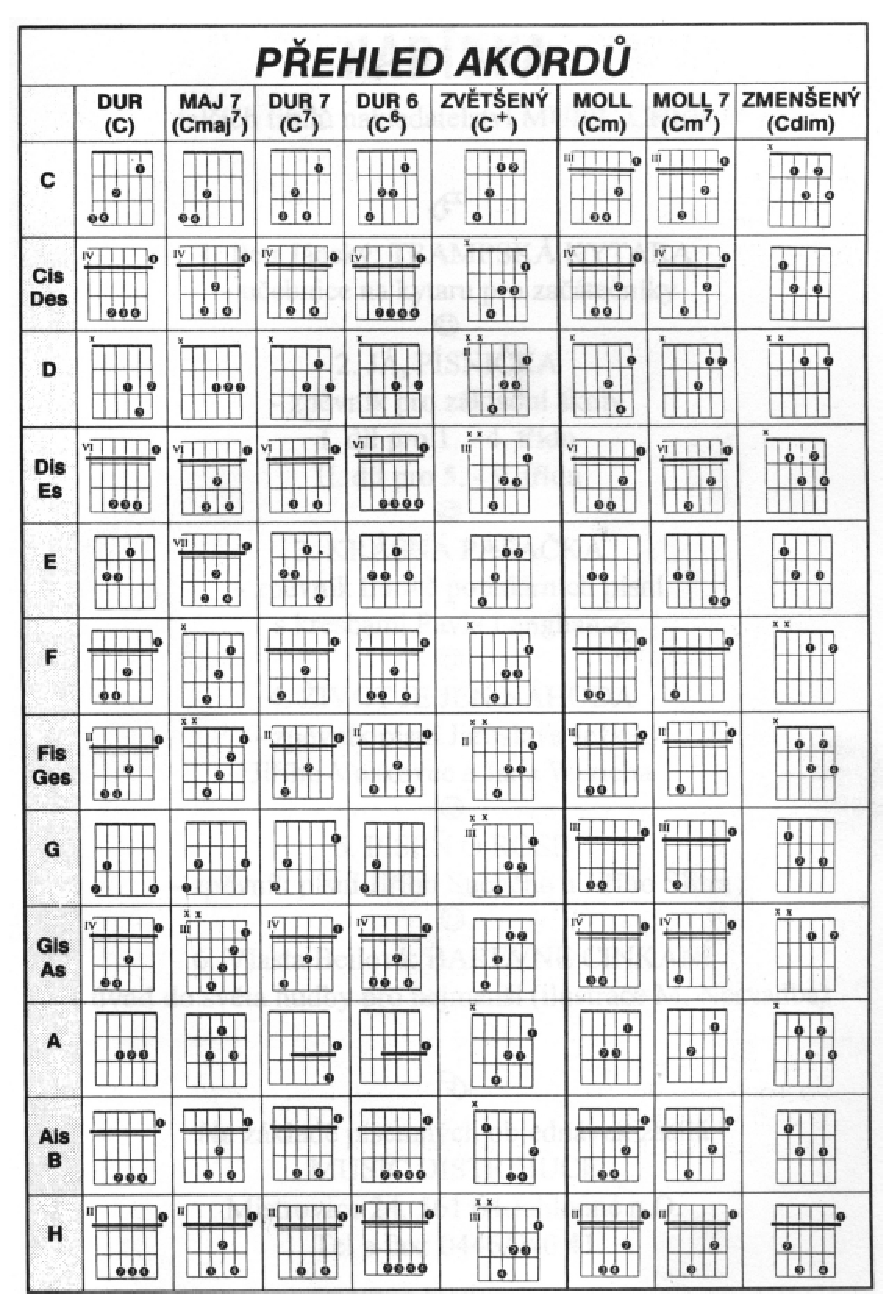
\includegraphics[height=\textheight]{../Akordy/AAAkordy3.pdf}
}
\end{figure}


\end{document}
